\begin{figure}[b]
  \centering
  \subfloat[$F_x$]{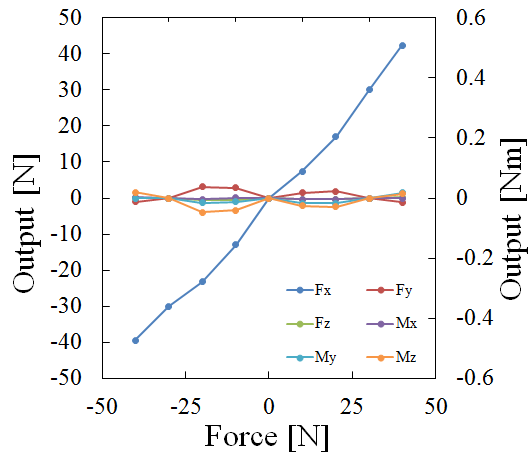
\includegraphics[scale=0.3]{pic/Fx_L.png}}
  \subfloat[$F_y$]{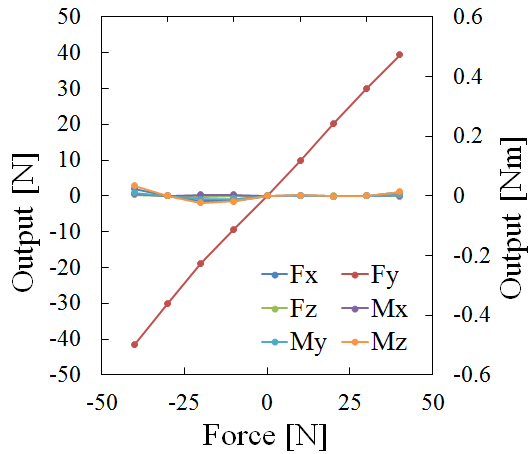
\includegraphics[scale=0.3]{pic/Fy_L.png}}\\
  \subfloat[$F_z$]{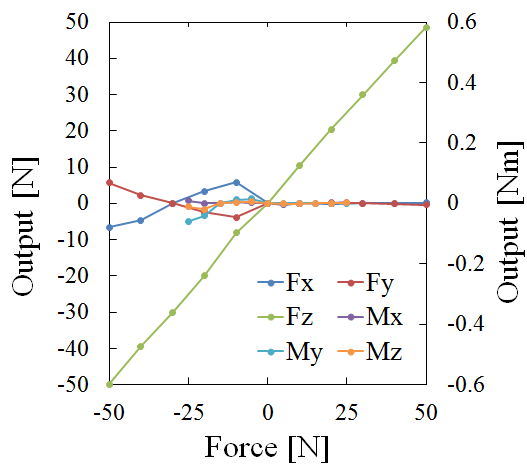
\includegraphics[scale=0.3]{pic/Fz_L.png}}
  \subfloat[$M_x$]{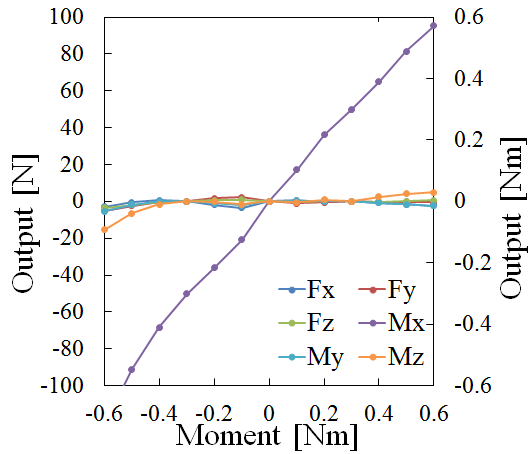
\includegraphics[scale=0.3]{pic/Mx_L.png}}\\
  \subfloat[$M_y$]{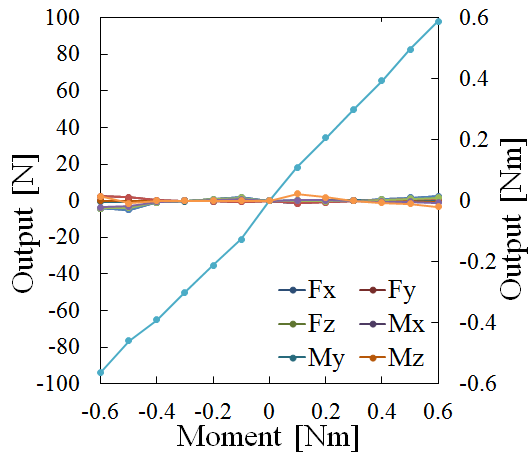
\includegraphics[scale=0.3]{pic/My_L.png}}
  \subfloat[$M_z$]{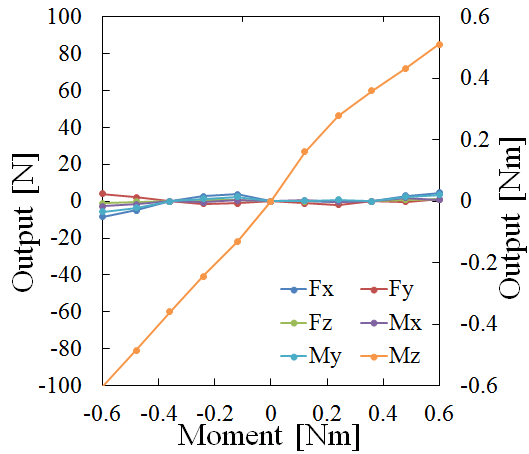
\includegraphics[scale=0.3]{pic/Mz_L.png}}\\
  \caption[]{荷重変換後の出力(低剛性起歪体)}\label{fig:kajyuLow}
\end{figure}
\begin{figure}[tb]
  \centering
  \subfloat[$F_x$]{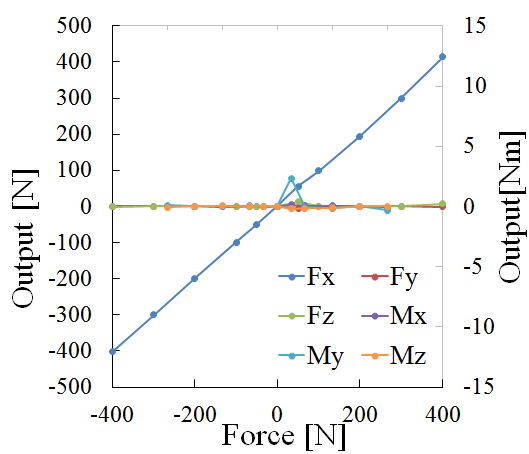
\includegraphics[scale=0.3]{pic/Fx_H.png}}
  \subfloat[$F_y$]{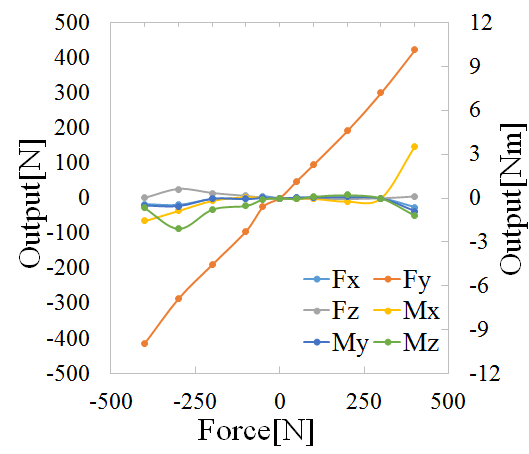
\includegraphics[scale=0.3]{pic/Fy_H.png}}\\
  \subfloat[$F_z$]{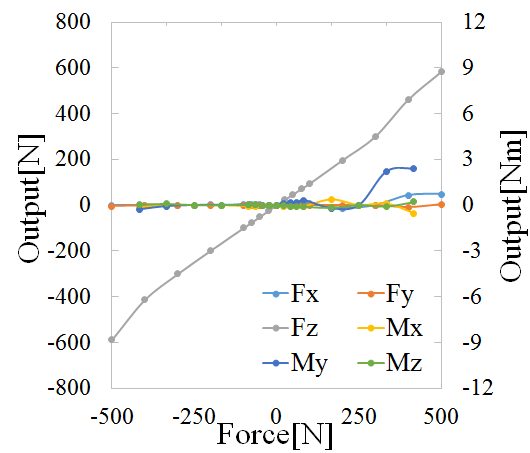
\includegraphics[scale=0.3]{pic/Fz_H.png}}
  \subfloat[$M_x$]{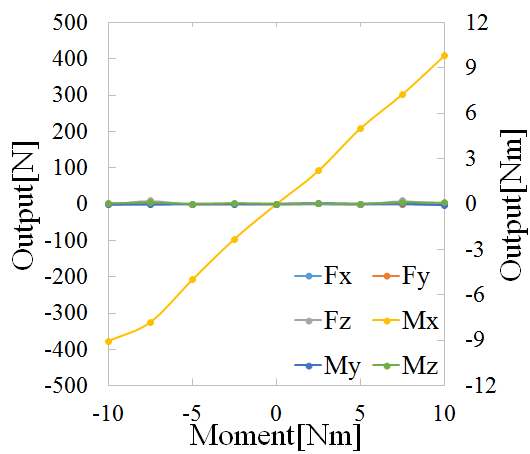
\includegraphics[scale=0.3]{pic/Mx_H.png}}\\
  \subfloat[$M_y$]{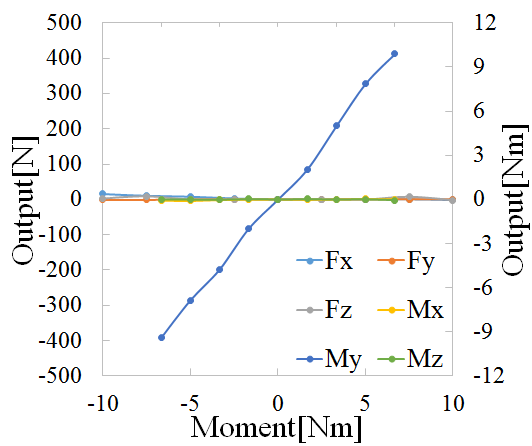
\includegraphics[scale=0.3]{pic/My_H.png}}
  \subfloat[$M_z$]{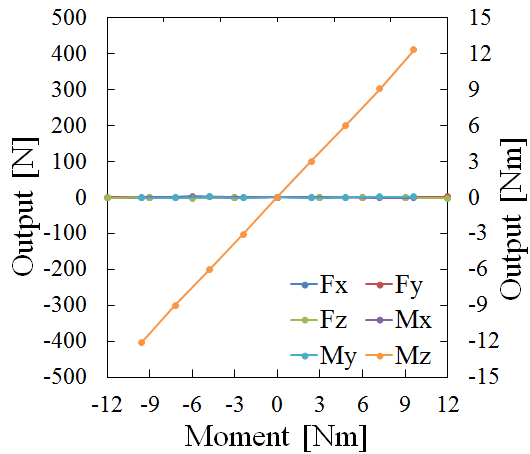
\includegraphics[scale=0.3]{pic/Mz_H.png}}\\
  \caption[]{荷重変換後の出力(高剛性起歪体)}\label{fig:kajyuHigh}
\end{figure}
\begin{figure}%[tb]
  \centering
  \subfloat[横軸:線形表示]{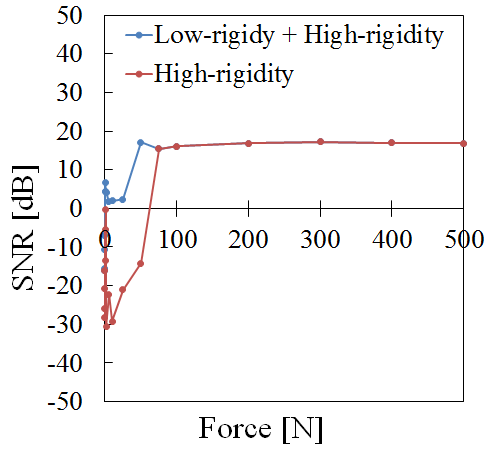
\includegraphics[scale=0.325]{pic/SN.png}}
  \subfloat[横軸:対数表示]{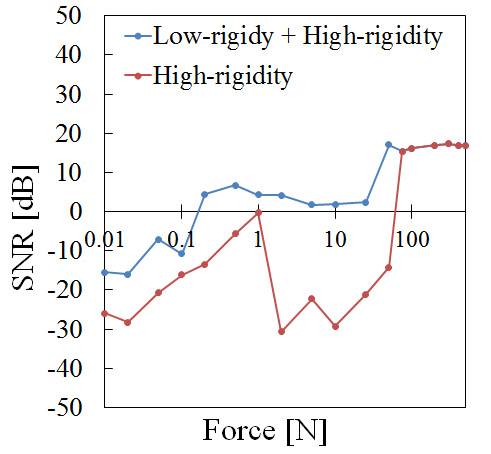
\includegraphics[scale=0.325]{pic/SNT.png}}\\
  \caption[]{SN比($F_z)$成分}\label{fig:sn}
\end{figure}
\begin{figure}%[tb]
  \centering
  \subfloat[低剛性起歪体]{\includegraphics[scale=0.325]{pic/1.png}}
  \subfloat[高剛性起歪体]{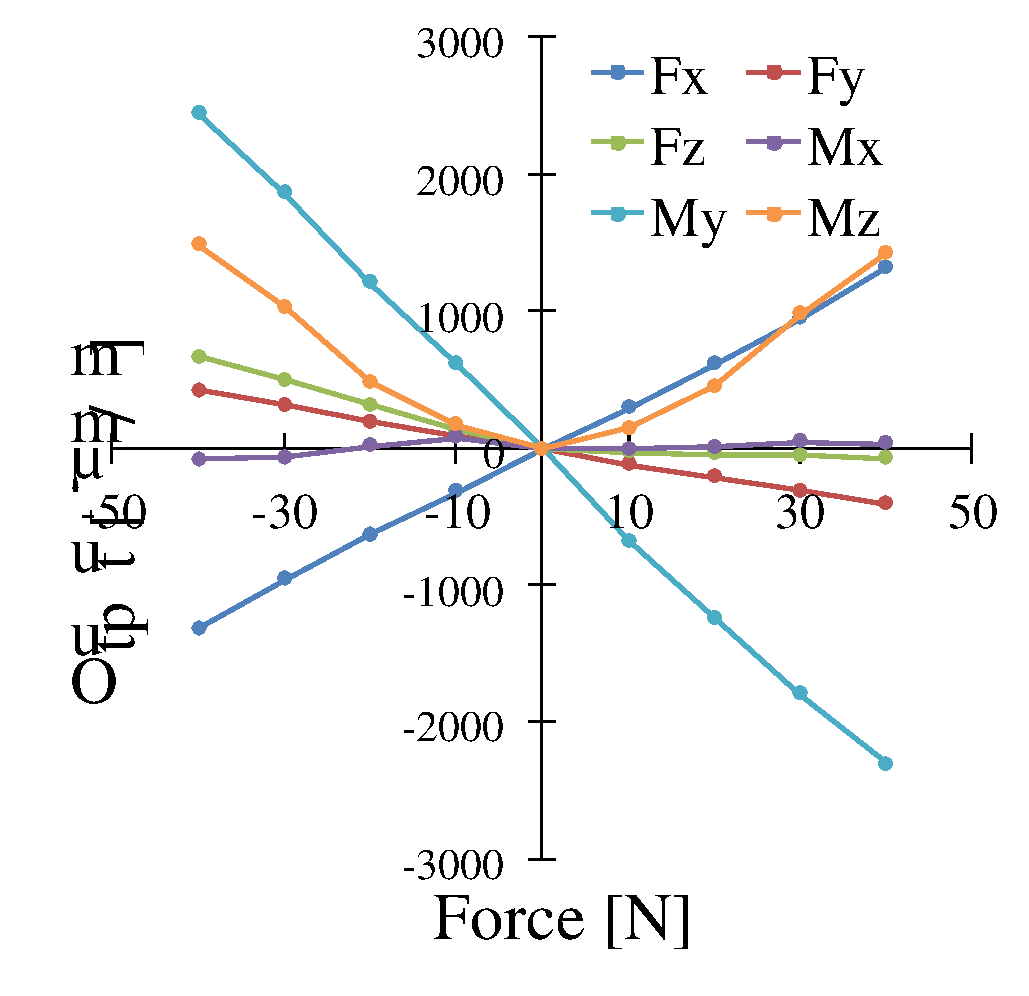
\includegraphics[scale=0.325]{pic/2.png}}\\
  \caption[]{$-F_z$を印加時のひずみ出力}\label{fig:stop}
\end{figure}
%\begin{figure}[tb]
 % \centering
 %\subfloat[$F_x$]{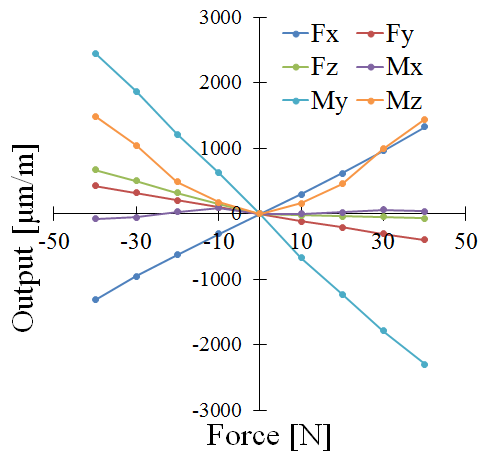
\includegraphics[scale=0.33]{pic/Sx_L.png}}
  %\subfloat[$F_y$]{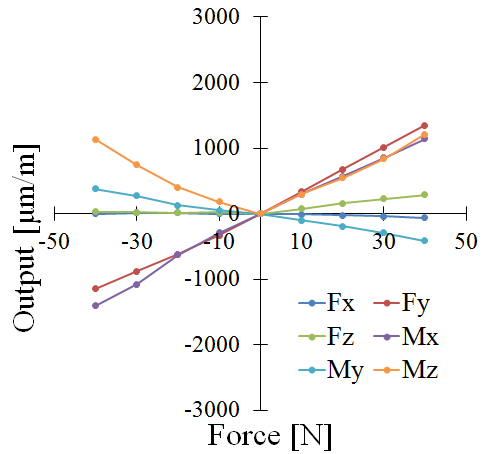
\includegraphics[scale=0.33]{pic/Sy_L.png}}\\
  %\subfloat[$F_z$]{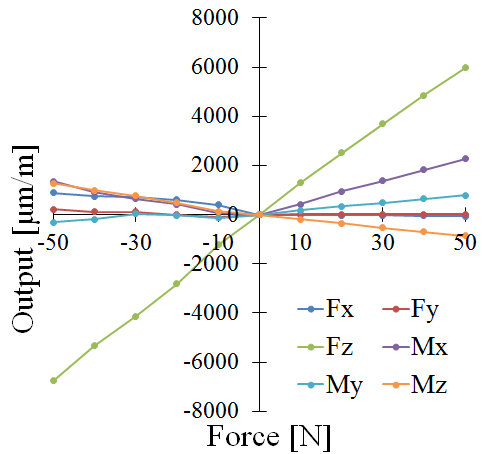
\includegraphics[scale=0.33]{pic/Sz_L.png}}
  %\subfloat[$M_x$]{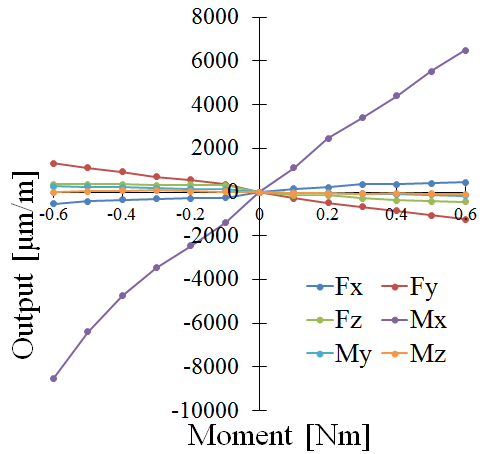
\includegraphics[scale=0.33]{pic/SMx_L.png}}\\
  %\subfloat[$M_y$]{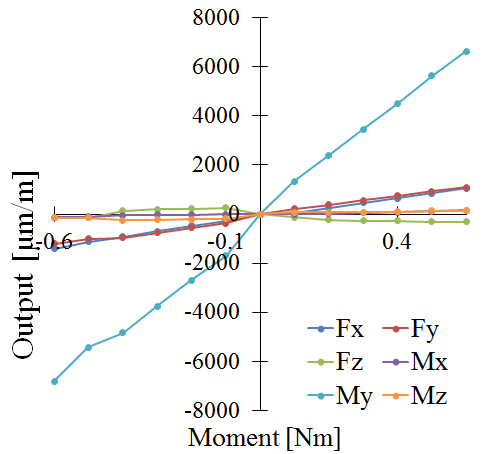
\includegraphics[scale=0.33]{pic/SMy_L.png}}
  %\subfloat[$M_z$]{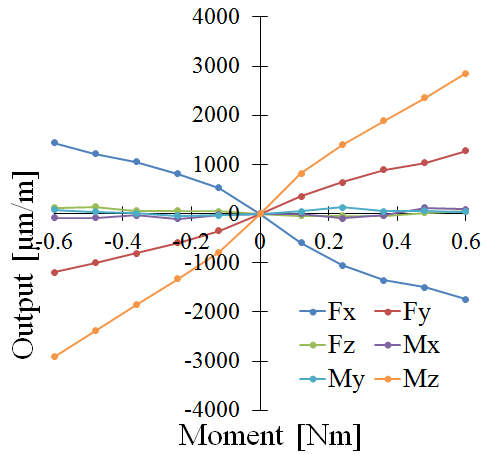
\includegraphics[scale=0.33]{pic/SMz_L.png}}\\
  %\caption[]{非線形性と他軸干渉(低剛性起歪体)}\label{fig:HTLow}
%\end{figure}
%\begin{figure}[tb]
 % \centering
 % \subfloat[$F_x$]{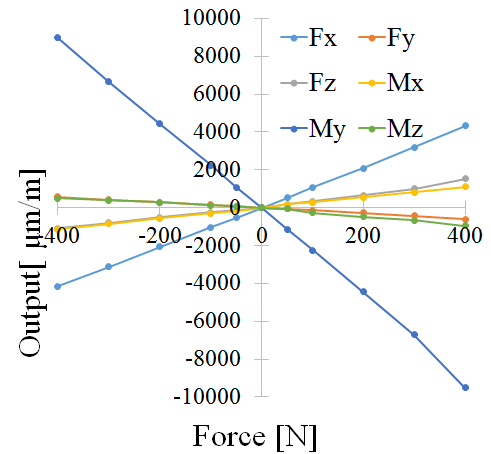
\includegraphics[scale=0.33]{pic/Sx_H.png}}
  %\subfloat[$F_y$]{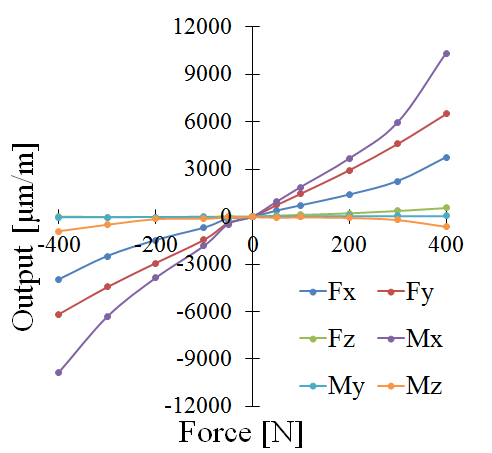
\includegraphics[scale=0.33]{pic/Sy_H.png}}\\
  %\subfloat[$F_z$]{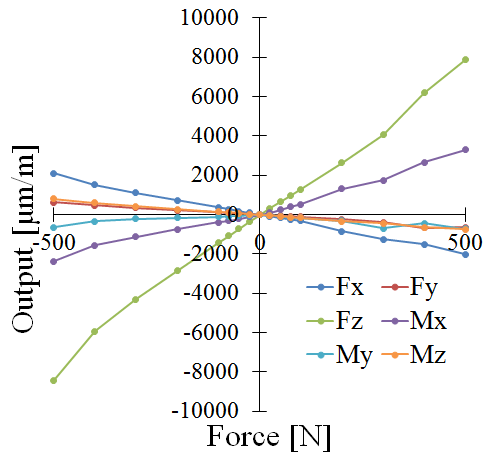
\includegraphics[scale=0.33]{pic/Sz_H.png}}
  %\subfloat[$M_x$]{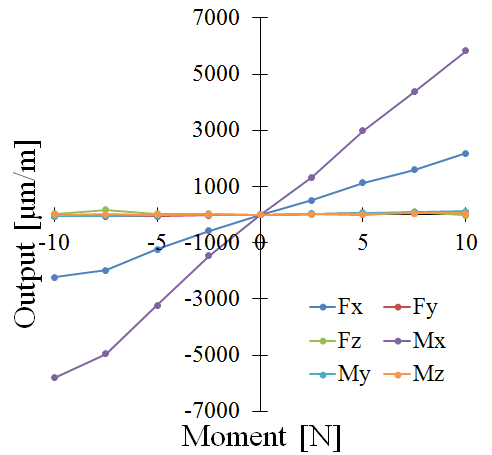
\includegraphics[scale=0.33]{pic/SMx_H.png}}\\
  %\subfloat[$M_y$]{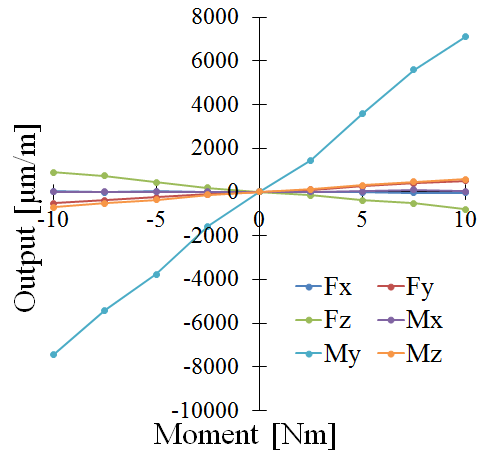
\includegraphics[scale=0.33]{pic/SMy_H.png}}
  %\subfloat[$M_z$]{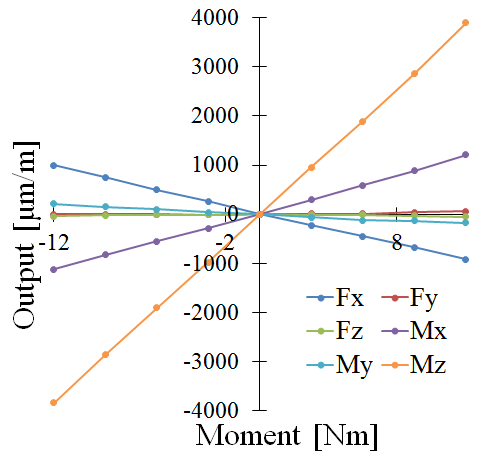
\includegraphics[scale=0.33]{pic/SMz_H.png}}\\
  %\caption[]{非線形性と他軸干渉(高剛性起歪体)}\label{fig:HTHigh}
%\end{figure}